\documentclass[a4paper,14pt]{extarticle}

\usepackage[T2A]{fontenc}
\usepackage[utf8]{inputenc}
\usepackage[english,russian]{babel}
\usepackage{indentfirst}
\usepackage{setspace}
\usepackage{geometry}
\geometry{a4paper,left=30mm,right=15mm,top=20mm,bottom=20mm}
\onehalfspacing
\setlength{\parindent}{1.25cm}

% Выравнивание заголовков по ГОСТ ИТМО
\usepackage{titlesec}
\titleformat{\section}[block]
{\centering\bfseries\Large}{\thesection}{1em}{}
\titleformat{\subsection}[block]
{\centering\bfseries\large}{\thesubsection}{1em}{}
\titleformat{\subsubsection}[block]
{\centering\bfseries\normalsize}{\thesubsubsection}{1em}{}

% Настройка подписей к рисункам по ГОСТ (номер и текст по центру)
\usepackage{caption}
\captionsetup[figure]{
    justification=centering,
    labelsep=endash,
    font=small,
    name=Рисунок,
    singlelinecheck=true
}

% Нумерация страниц по ГОСТ (снизу по центру)
\usepackage{fancyhdr}
\pagestyle{fancy}
\fancyhf{}
\fancyfoot[C]{\hspace{-15mm}\thepage}
\renewcommand{\headrulewidth}{0pt}

% Формат списков по ГОСТ
\usepackage{enumitem}
\setlist{nosep, leftmargin=1.25cm}
\setlist[itemize]{label=\raisebox{0.3ex}{\tiny$\bullet$}, labelsep=0.5em}

% Ссылки и математика
\usepackage{hyperref}
\hypersetup{
    colorlinks=true,
    linkcolor=black,
    urlcolor=black,
    citecolor=black
}
\usepackage{amsmath}
\usepackage{graphicx}

% Разрешить более свободный перенос длинных строк
\sloppy

% Команды для удобства
\newcommand{\sectionbreak}{\clearpage}
\newcommand{\img}[3]{%
    \begin{figure}[H]
    \centering
    \includegraphics[width=#1\textwidth]{#2}
    \caption{#3}
    \label{fig:#2}
    \end{figure}
}

\begin{document}
    \thispagestyle{empty}
    \begin{center}
    {\Large\textbf{ФЕДЕРАЛЬНОЕ ГОСУДАРСТВЕННОЕ АВТОНОМНОЕ ОБРАЗОВАТЕЛЬНОЕ УЧРЕЖДЕНИЕ ВЫСШЕГО ОБРАЗОВАНИЯ}}
        \\
        {\Large\textbf{«НАЦИОНАЛЬНЫЙ ИССЛЕДОВАТЕЛЬСКИЙ УНИВЕРСИТЕТ ИТМО»}}\\[5mm]
        {\large ФАКУЛЬТЕТ ТЕХНОЛОГИЙ ИСКУССТВЕННОГО ИНТЕЛЛЕКТА}\\[5mm]
        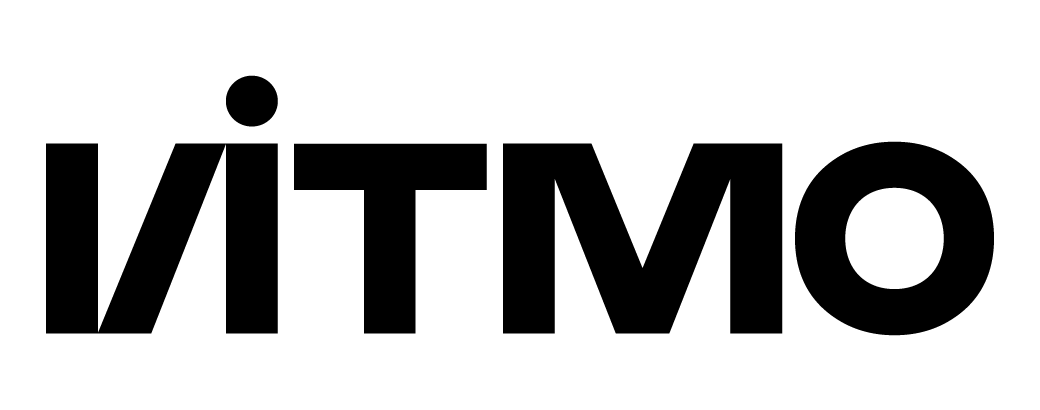
\includegraphics[scale=0.14]{logo.png}\\[10mm]
        \rule{\textwidth}{0.4mm}\\[3mm]
        {\Large Расчётно-графическая работа \textnumero{} 1 }\\[3mm]
        {\Large по дисциплине «Теория вероятностей }\\[3mm]
        {\Large и продвинутая математическая статистика» }\\[3mm]
        \rule{\textwidth}{0.4mm}
    \end{center}
    \vfill
    \begin{flushright}
        \large Выполнили студенты группы J3211: \\
        Воробьев А.П. \\
        ИСУ: 465440 \\
        Шакина А.С. \\
        ИСУ: 396675 \\
        Преподаватель практики: \\
        Кононов И.А.
    \end{flushright}
    \vfill
    \begin{center}
        \large Санкт-Петербург \\
        \large 2025
    \end{center}
    \newpage


% =============================================
% Задача 1
% =============================================
    
    
    \section*{Задача 1}
        
        \subsection*{Постановка задачи}
            
            Требуется аналитически решить задачу. Помимо этого нужно написать программу, которая будет считать данные вероятности приблизительно с помощью метода Монте-Карло. Особо любознательные могут задаться поиском (аналитическим) оптимального количества итераций, которых будет достаточно для получения ответа с достаточно «разумной» точностью. При решении задач могут быть полезны принципы произведения вероятностей и включений-исключений.
        
        \subsection*{Условие варианта 2}
            
            В городе живут \( n + 1 \) людей. Человек, условный «прародитель», пишет два письма случайно выбранным адресатам, которые образуют «первое» поколение. Те делают то же самое, в результате чего образуется «второе поколение». В общем, на каждое полученное письмо горожанин готовит два ответа и отправляет двум случайным жителям. Найти вероятность того, что прародитель не входит ни в одно из поколений с номерами \( 1 \ldots r \).
        
        \subsection*{Аналитическое решение}
            
            \subsubsection*{Обозначения и допущения}
                
                Обозначения:
                \begin{itemize}
                    \item \( n + 1 \) - количество жителей города.
                    \item \( r \) - количество поколений, которые мы рассматриваем.
                    \item \( S_i \) - число входящих писем в поколении \( i \).
                    \item \( A \) - событие, что прародитель не является адресатом письма
                \end{itemize}
                
                Допущение: Отправитель письма не может быть его адресатом.
            
            \subsubsection*{Решение}
                
                Рассмотрим \( i \)-е поколение.
                Каждое входящее письмо порождает два исходящих, которые отправляются двум случайным жителям города (кроме самого отправителя). Так как в первом поколении - \( S_1 = 2 \) письма, то во втором поколении будет \( S_2 = 2 \cdot S_1 = 4 \) и так далее. Таким образом, количество писем в \( i \)-м поколении можно выразить формулой:
                \[
                    S_i = 2 \cdot S_{i-1} = 2^i
                \]
                
                Заметим, что в первом поколении не может быть прародителя, поэтому количество писем \( M \) за \( r \) поколений, адресатом для которого может быть прародитель, равно:
                \[
                    M = \sum_{i=2}^{r} S_i = \sum_{i=2}^{r} 2^i = 2^{r+1} - 4
                \]
                
                Теперь найдем вероятность \( P(A) \), что прародитель не является адресатом одного письма. Так как отправитель не может быть адресатом, то для каждого письма есть \( n \) возможных адресатов, из которых \( n - 1 \) не являются прародителем. Значит:
                \[
                    P(A) = \frac{n - 1}{n}
                \]
                
                Так как все адресаты выбираются независимо, то вероятность \( P (A_M) \), что прародитель не является адресатом ни одного из \( M \) писем:
                \[
                    P(A_M) = P(A)^M = \left(\frac{n - 1}{n}\right)^{2^{r+1} - 4}
                \]
            
            \subsubsection*{Ответ}
                
                Таким образом, искомая вероятность, что прародитель не входит ни в одно из поколений с номерами \( 1 \ldots r \), равна:
                \[
                    \boxed{P(A_M) = \left(\frac{n - 1}{n}\right)^{2^{r+1} - 4}}
                \]
        
        \subsection*{Приближённое решение методом Монте-Карло}
            
            Решение методом Монте-Карло реализовано в блокноте \href{https://github.com/vorandpav/TVIPS}{1.ipynb}.


% =============================================
% Задача 2
% =============================================
    
    
    \section*{Задача 2}
        
        \subsection*{Постановка задачи}
            
            Тоже как и в первом упражнении нужно решить аналитически и написать скрипт, вычисляющий вероятность приближенно по методу Монте-Карло. Дополнительный вопрос о поиске числа итерация тоже имеет место быть.
        
        \subsection*{Условие варианта 2}
            
            На отрезке длины l независимо одна от другой поставлены две точки, положение каждой из которых равновозможно на этом отрезке. Определить вероятность того, что из трех получившихся частей одного отрезка можно построить треугольник.
        
        \subsection*{Аналитическое решение}
            
            \subsubsection*{Упрощения и обозначения}
                Обозначения:
                \begin{itemize}
                    \item \( x, y \) - случайные величины, соответствующие координатам точек на отрезке.
                    \item \( u = min(x, y) \), \( v = max(x, y) \) - упорядоченные координаты точек.
                    \item \( a = u \), \( b = v - u \), \( c = 1 - v \) - длины отрезков, на которые разбиваются исходный отрезок.
                    \item \( A \) - событие, что из отрезков можно построить треугольник.
                \end{itemize}
                
                Упрощения:
                \begin{itemize}
                    \item Без потери общности можно считать, что \( l = 1 \), так как вероятность не зависит от длины отрезка.
                    \item Две точки на отрезке можно рассматривать, как координаты на единичном квадрате \( [0, 1] \times [0, 1] \).
                    \item Поскольку пары \( (x, y) \) и \( (y, x) \) приводят к одинаковым отрезкам, то можно рассматривать только половину квадрата, где \( x \leq y \). Площадь этой половины равна \( \frac{1}{2} \).
                \end{itemize}
            
            \subsubsection*{Решение}
                
                Из всего вышесказанного, мы имеем, что \( x = u \), \( y = v \), \( 0 \leq x \leq y \leq 1 \), \(a = x\), \(b = y - x\), \(c = 1 - y\). Событие \( A \) - соблюдение неравенств треугольника можно записать как:
                \[
                    \begin{cases}
                        a + b > c
                        \leftrightarrow
                        x + (y - x) > 1 - y
                        \leftrightarrow
                        y > \frac{1}{2} \\
                        a + c > b
                        \leftrightarrow
                        x + (1 - y) > y - x
                        \leftrightarrow 2x + 1 > 2y
                        \\
                        b + c > a
                        \leftrightarrow
                        (y - x) + (1 - y) > x
                        \leftrightarrow
                        1 - x > x
                        \leftrightarrow
                        x < \frac{1}{2}
                    \end{cases}
                \]
                
                С учётом ограничений \( 0 \leq x \leq y \leq 1 \), получаем систему неравенств:
                \[
                    \begin{cases}
                        0 \leq x < \frac{1}{2} \\
                        \frac{1}{2} < y \leq 1 \\
                        x \leq y \\
                        y < x + \frac{1}{2}
                    \end{cases}
                \]
                
                Построим область, удовлетворяющую системе неравенств:
                
                Найдём область \( S_A \), удовлетворяющую системе неравенств.
                \[
                    S_A =
                    \int_{x = 0}^{x = \frac{1}{2}}
                    \int_{y = \frac{1}{2}}^{y = x + \frac{1}{2}} dy dx =
                    \int_{x = 0}^{x = \frac{1}{2}}
                    ((x + \frac{1}{2}) - \frac{1}{2}) dx =
                    \int_{x = 0}^{x = \frac{1}{2}} x dx =
                    \frac{1}{8} - 0 = \frac{1}{8}
                \]
                
                Таким образом, вероятность \( P(A) \) равна отношению площади \( S_A \) к площади треугольной области, которая равна \( \frac{1}{2} \):
                \[
                    P(A) = \frac{S_A}{\frac{1}{2}} = \frac{\frac{1}{8}}{\frac{1}{2}} = \frac{1}{4}
                \]
            
            \subsubsection*{Ответ}
                Таким образом, искомая вероятность, что из трёх частей отрезка можно построить треугольник, равна:
                \[
                    \boxed{P(A) = \frac{1}{4}}
                \]
        
        \subsection*{Приближённое решение методом Монте-Карло}
            Решение методом Монте-Карло реализовано в блокноте \href{https://github.com/vorandpav/TVIPS}{2.ipynb}.


% =============================================
% Задача 3
% =============================================
    
    
    \section*{Задача 3}
        
        \subsection*{Постановка задачи}
            
            Требуется аналитически решить задачу.
        
        \subsection*{Условие варианта 2}
            
            Введём события \( A_i = \{X = i\}, B_i = \{Y = i\}, i \geq 0 \). Известно, что для любых \( i \geq 0, j \geq 0 \) события \( A_i \) и \( B_j \) -- независимы, при этом
            \[ P(X = i) = e^{-\lambda} \frac{\lambda^i}{i!}, \lambda > 0, i \geq 0, \]
            \[ P(Y = j) = e^{-\mu} \frac{\mu^j}{j!}, \mu > 0, i \geq 0. \]
            Требуется найти \( P(X = i | X + Y = j) \).
        
        \subsection*{Решение}
            
            Для нахождения вероятности \( P(X = i | X + Y = j) \) используем формулу условной вероятности:
            \[ P(A|B) = \frac{P( A \cap B)}{P(B)}, \]
            причём \(A = \{X = i\}, B = \{X + Y = j\}\).
            
            Найдём \(P( A \cap B)\). Пересечение событий означает, что что \(X\) должно быть равно \(i\), и одновременно \(X+Y\) должно быть равно \(j\). Это возможно только если \(Y=j-i\).
            
            Таким образом, событие \(\{X = i \cap X + Y = j\}\) эквивалентно событию \(\{X = i \cap Y = j - i\}\). Подставим в формулу:
            \[P(A \cap B ) =  e^{-\lambda} \frac{\lambda^i}{i!} \cdot e^{-\mu} \frac{\mu^{j-i}}{(j-i)!} = e^{-(\lambda + \mu)} \cdot \frac{\lambda^i \mu^{j-i}}{i!(j-i)!}\]
            
            Найдём \(P(B) = P(X + Y = j) \). Запишем событие \(\{X + Y = j\}\) как \(\{X = k \cap Y = j-k\} \;\; \forall k \in {1, \dots, j}\). Так как события несовместны и независимы:
            \[ P(X + Y = j) = \sum_{k=0}^{j} P(X = k \cap Y = j-k) = \sum_{k=0}^{j}P(X = k) P(Y = j - k)\]
            
            По условию:
            \[P(X = k) = e^{-\lambda} \frac{\lambda^k}{k!}, \; P(Y = j - k) = e^{-\mu} \frac{\mu^{j-k}}{(j-k)!}, \]
            тогда
            \[ P(X + Y = j) = e^{-(\lambda + \mu)} \sum_{k=0}^{j} \frac{\lambda^k \mu^{j-k}}{k!(j-k)!} \]
            
            Воспользуемся биномом Ньютона: \[(\lambda + \mu)^j = \sum_{k=0}^{j} \frac{j!}{k!(j-k)!} \lambda^k \mu^{j-k}\]
            
            Следовательно:
            \[P(X+Y=j) = e^{-(\lambda + \mu)} \frac{(\lambda+\mu)^j}{j!}.\]
            
            Подставим полученные выражения в формулу условной вероятности:
            \[P(A|B) = \frac{P( A \cap B)}{P(B)} = \frac{e^{-(\lambda + \mu)} \frac{\lambda^i \mu^{j-i}}{i!(j-i)!}}{e^{-(\lambda + \mu)} \frac{(\lambda+\mu)^j}{j!}} = \frac{j!}{i!(j-i)!} \cdot \frac{\lambda^i \mu^{j-i}}{(\lambda+\mu)^j} =\]
            \[ = C_j^i \cdot \big(\frac{\lambda}{\lambda+\mu}\big)^i \cdot \big(\frac{\mu}{\lambda+\mu}\big)^{j-i}\]
            
            \subsubsection*{Ответ}
                
                Таким образом, искомая вероятность равна:
                \[
                    \boxed{C_j^i \cdot \big(\frac{\lambda}{\lambda+\mu}\big)^i \cdot \big(\frac{\mu}{\lambda+\mu}\big)^{j-i}}
                \]


% =============================================
% Задача 4
% =============================================
    
    
    \section*{Задача 4}
        
        \subsection*{Постановка задачи}
            
            Представьте, что вам нужно быстро создать некий программный продукт, в котором будут использоваться вероятностные модели. Возможно, вы будете использовать Python и модуль \texttt{SciPy}, в котором реализовано достаточно много математических алгоритмов и моделей, в том числе и вероятностно-статистических (подмодуль \texttt{stats}). Допустим, в вашей модели есть ``нестандартное'' распределение (например, не реализованное в \texttt{SciPy}), для которого известна плотность, и вам нужно быстро реализовать распределение, то есть определить функцию распределения, квантили и прочие методы. Тогда идея унаследоваться от класса \texttt{rv\_continuous} кажется разумной: ведь достаточно переопределить метод, соответствующий плотности. Казалось бы, отличная идея, плюс применили объектно-ориентированный подход. Но допустим, что вам понадобилось сгенерировать случайные числа (на самом деле псевдослучайные) из данного распределения, но вдруг что-то пойдёт не так, например, будет слишком долго работать... И вдруг нужно будет сообразить другие методы.
            
            \textit{Само задание:}
            \begin{enumerate}
                \item Для заданной плотности $p$ наследуйтесь от класса \texttt{rv\_continuous} и сгенерируйте с помощью реализованного подкласса для вашего распределения $n$ случайных чисел из данного распределения. Посмотрите, как будет работать алгоритм при росте $n$ (сразу большим $n$ не делайте). Убедитесь эмпирически, что распределение сгенерированных чисел согласуется с данным вероятностным законом.
                \item Реализуйте генерацию для вашего распределения с помощью обратной к функции распределения (при написании функции для $F^{-1}$ вызов специальных функций, например, квантили стандартного нормального закона разрешается; не забыть аналитический вывод $F^{-1}$). Проведите тот же эксперимент.
                \item Выберите ещё один метод для генерации случайных чисел (можно, например, rejecting sampling, ratio of uniforms или другой метод). Опишите его математическое обоснование. Воспользуйтесь реализацией или сами реализуйте. Проведите тот же эксперимент.
            \end{enumerate}
        
        \subsection*{Условие варианта 2}
            
            \[
                p(x) = 3x^2 e^{-x^3} \cdot 1(x \geq 0)
            \]
        
        \subsection*{Аналитические вычисления}
            
            \subsubsection*{Плотность распределения}
                \[
                    p(x) = 3x^2 e^{-x^3} \cdot 1(x \geq 0)
                \]
            
            \subsubsection*{Функция распределения}
                \[
                    F(x) =
                    \int_{-\infty}^{x} p(t) dt =
                    \int_{0}^{x} 3t^2 e^{-t^3} dt =
                    -e^{-t^3} \Big|_{0}^{x} =
                    1 - e^{-x^3}
                \]
                То есть:
                \[
                    F(x) = \begin{cases}
                               0, & x < 0 \\
                               1 - e^{-x^3}, & x \geq 0
                    \end{cases}
                \]
            
            \subsubsection*{Обратная функция распределения}
                \[
                    F(x) = 1 - e^{-x^3} \leftrightarrow
                    1 - F(x) = e^{-x^3} \leftrightarrow
                    \ln(1 - F(x)) = -x^3 \leftrightarrow
                    x = (-\ln(1 - F(x)))^{1/3}
                \]
                Тогда обратная функция распределения:
                \[
                    F^{-1}(y) = (-\ln(1 - y))^{1/3}, \quad y \in [0, 1)
                \]
            
            \subsubsection*{Метод rejection sampling}
                
                \paragraph{Идея метода}
                    Генерация семплов по $f(x)$ происходит с помощью более простого вспомогательного распределения $g(x)$, которое мы можем просемплировать, и которое удовлетворяет следующему условию:
                    \[
                    \forall x \ f(x)<cg(x), \quad c > 1
                    \]
                
                \paragraph{Алгоритм}
                    \begin{enumerate}
                            \item Взять семпл $x$ по распределению $g(x)$;
                            \item Выбрать случайное число $u$ равномерно из отрезка $[0,cg(x)]$;
                            \item Вычислить $f(x)$;
                            \item Если $u \leq f(x)$, то $x$ добавляется к семплам;
                            \item Если $u > f(x)$, то $x$ отклоняется (отсюда и название метода).
                    \end{enumerate}
                
                \paragraph{Обоснование}
                    Пусть $Y$ — случайная величина с плотностью распределения $g(y)$, а $U$ — случайная величина, равномерно распределённая на отрезке $[0, cg(x)]$.
                    
                    Мы хотим показать, что условная плотность $Y$ при условии события $U \leq f(Y)$ равна искомой плотности $f(x)$.
                    \[
                    P(Y = y \mid U \leq f(Y)) =
                    \frac{P(Y = y \cap U \leq f(Y))}{P(U \leq f(Y))}
                    \]
                    
                    Рассмотрим знаменатель. Заметим, что $U$ и $Y$ независимы, так как $U$ выбирается независимо от $Y$.
                    \begin{gather*}
                            P(A) =
                            P(U \leq f(Y)) =
                            \int_{-\infty}^{\infty} P(U \leq f(y)) g(y) dy =\\
                            = \int_{-\infty}^{\infty} \frac{f(y)}{cg(y)} g(y) dy =
                            \frac{1}{c} \int_{-\infty}^{\infty} f(y) dy =
                            \frac{1}{c}
                    \end{gather*}
                    
                    Рассмотрим числитель.
                    \begin{gather*}
                            P(Y = y \cap U\le f(Y)) = P(U\le f(Y) | Y = y) \cdot P (Y = y) =\\
                            = P(U\le f(y)) \cdot g(y) =
                            = \frac{f(y)}{cg(y)}g(y) = \frac{f(y)}{c}
                    \end{gather*}
                    
                    Теперь объединим и получим искомый результат:
                    \[
                    P(Y=y|U\le f(Y)) =
                    \frac{f(y)}{c}\cdot c = f(y)
                    \]
                
                \paragraph{Выбор вспомогательного распределения}
                    
                    В качестве вспомогательного распределения выберем экспоненциальное распределение $g(x) = e^{-x}$.
                    Для метода необходимо найти константу $c$ такую, что $p(x) \leq c \cdot g(x)$ для всех $x \geq 0$.
                    Это эквивалентно поиску максимума функции $h(x) = \frac{p(x)}{g(x)}$:
                    \[
                    h(x) = \frac{3x^2 e^{-x^3}}{e^{-x}} = 3x^2 e^{x - x^3}
                    \]
                    
                    Найдём производную $h(x)$, чтобы найти её максимум:
                    \begin{gather*}
                            h'(x) = 6x e^{x - x^3} + 3x^2 e^{x - x^3} (1 - 3x^2) = \\
                            = 3x e^{x - x^3} (2 + x(1 - 3x^2)) = 3x e^{x - x^3} (2 + x - 3x^3)
                    \end{gather*}
                    
                    Приравняем производную к нулю, чтобы найти критические точки, $x \geq 0$:
                    \begin {gather*}
                            3x e^{x - x^3} (2 + x - 3x^3) = 0 \leftrightarrow
                            x = 0 \lor (x-1)(3x^2 + 3x + 2) = 0 \leftrightarrow \\
                            \leftrightarrow x = 0 \lor x = 1
                    \end{gather*}
                    
                    \begin{itemize}
                            \item При $x=0$, $h(0) = 0$.
                            \item При $x=1$, $h(1) = 3(1)^2 e^{1-1} = 3$.
                    \end{itemize}
                    
                    Поскольку $\lim_{x \to \infty} h(x) = 0$, максимум функции достигается в точке $x=1$.
                    Таким образом, можно выбрать $c = 3$.
        
        \subsection*{Эмпирическое решение и выводы}
            Эксперименты, их результаты и выводы написаны блокноте \href{https://github.com/vorandpav/TVIPS}{4.ipynb}.

    \section*{Задача 5}
        \subsection*{Постановка задачи}
            
            Для заданного распределения требуется найти:
            \begin{itemize}
                \item "нормирующие" константы;
                \item функцию распределения;
                \item математическое ожидание, дисперсию, среднее квадратическое отклонение, моду, медиану, асимметрию, эксцесс
                \item функцию распределения и плотность функции от исходной случайной величины
            \end{itemize}
        
        \subsection*{Условие варианта 5}
        \[p_X(x) = c \cos x \cdot ind(x \in \big[-\frac{\pi}{2}, \frac{\pi}{2}\big]), Y = \sin X\]
        
        \subsection*{Решение}
        \noindent 1. Найдём нормирующую константу $c$. 

        Так как $p_X(x)$ -- плотность, то $\int_{-\pi/2}^{\pi/2} p_X(x) dx = 1$. Подставим:
        \[\int_{-\pi/2}^{\pi/2} c \cos x dx = 1\]
        \[c \sin x |^{\pi/2}_{-\pi/2} = 1\]
        \[c(\sin(\pi/2) - \sin(-\pi/2)) = 1\]
        \[c(1 - (-1)) = 1 \implies 2c = 1 \implies \boxed{c = \frac{1}{2}}\]
        
        \noindent 2. Найдём функцию распределения:
        \[F_X(x) = \int_{-\pi/2}^{\pi/2}\frac{1}{2}\cos t dt = \frac{1}{2} (\sin x + 1). \]
        
        Тогда: \[ \boxed{F_X (x)= \begin{cases}
            0, & x < -\frac{\pi}{2} \\
            \frac{1}{2} (\sin x + 1), & -\frac{\pi}{2} < x < \frac{\pi}{2} \\
            1, & x > \frac{\pi}{2}
        \end{cases}}\] 

        \noindent 3. Математическое ожидание:
        \[E[X] = \int_{-\infty}^{\infty} x \cdot p_X(x) dx\]
        \[E[X] = \int_{-\pi/2}^{\pi/2} x \cdot \frac{1}{2} \cos x dx\]
        Подынтегральная функция является нечётной, а интегра по симметричному промежутку от нечётной функции равен нулю:
        \[\boxed{E[X] = 0}\]

        Дисперсия:
        \[D[X] = E[X^2] - (E[X])^2\]
        Так как $E[X] = 0$, то $D[X] = E[X^2]$. 
        \[E[X^2] = \int_{-\pi/2}^{\pi/2} x^2 \cdot \frac{1}{2} \cos x dx\]
        Так как подынтегральная функция -- чётная: \[E[X^2] = 2 \cdot \frac{1}{2} \int_{0}^{\pi/2} x^2 \cos x dx = \int_{0}^{\pi/2} x^2 \cos x dx\]
        \\ Два раза интегрируем по частям:
        \begin{gather*}
            u = x^2, dv = \cos x dx \implies du = 2x dx, v = \sin x \\
            \int_{0}^{\pi/2} x^2 \cos x dx = x^2 \sin x dx |^{\pi/2}_{0} - \int_{0}^{\pi/2} 2x \sin x dx = \\ 
            = \frac{\pi^2}{4} - 2 \int_{0}^{\pi/2} x \sin x dx 
        \end{gather*}
        \begin{gather*}
            u = x, dv = \sin x dx \implies du = dx, v = -\cos x \\
            \int_{0}^{\pi/2} x \sin x dx = -x \cos x |^{\pi/2}_0 - \int_{0}^{\pi/2} (-\cos x) dx = \\
            = (-\frac{\pi}{2} \cdot 0 - 0) + (\sin x |^{\pi/2}_0) = 0 + (\sin \frac{\pi}{2} - \sin 0) = 1 - 0 = 1
        \end{gather*}
        Подставим обратно: 
        \[\boxed{D[X] = E[X^2] = \frac{\pi}{4} - 2 \cdot 1 = \frac{\pi}{4} - 2}\]

        Среднее квадратическое отклонение:
        \[\boxed{\sigma_X = \sqrt{D[X]} = \sqrt{\frac{\pi}{4} - 2}}\]

        Мода:
        \[\boxed{mod_X = \arg \max_x p_X(x) = \arg \max_x \frac{1}{2} \cos x = 0}\]

        Медиана: 
        $$
        med = \arg\min_a E[|X - a|] = \arg\min_a \int_{-\infty}^{\infty} |x - a| p_X(x) dx
        $$
        Для данной плотности $p_X(x) = \frac{1}{2} \cos x \cdot ind\left(x \in \left[-\frac{\pi}{2}, \frac{\pi}{2}\right]\right)$, функция для минимизации:
        $$
        g(a) = \int_{-\pi/2}^{\pi/2} |x - a| \cdot \frac{1}{2} \cos x dx
        $$

        Минимум достигается при $g'(a) = 0$. Дифференцируем $g(a)$ по $a$:
        $$
        g'(a) = \frac{1}{2} \left( \int_{-\pi/2}^{a} \cos x dx - \int_{a}^{\pi/2} \cos x dx \right)
        $$

        Приравниваем производную к нулю:
        \begin{align*}
        g'(a) = 0 &\implies \int_{-\pi/2}^{a} \cos x dx = \int_{a}^{\pi/2} \cos x dx \\
        & \sin x|_{-\pi/2}^{a} = \sin x|_{a}^{\pi/2} \\
        & \sin a - \sin\left(-\frac{\pi}{2}\right) = \sin\left(\frac{\pi}{2}\right) - \sin a \\
        & \sin a - (-1) = 1 - \sin a \\
        & \sin a + 1 = 1 - \sin a \\
        &   \sin a = 0 \\
        & \sin a = 0
        \end{align*}
        Единственное решение для $a \in \left[-\frac{\pi}{2}, \frac{\pi}{2}\right]$:
        $$
        a = 0
        $$
        Следовательно:
        $$
        \boxed{med = 0}
        $$

        Коэффициент асиммерии:
        $$
        As = \frac{E[(X - E[X])^3]}{\sigma_X^3}
        $$

        Поскольку $E[X] = 0$:
        $$
        E[(X - E[X])^3] = E[X^3] = \int_{-\pi/2}^{\pi/2} x^3 \cdot p_X(x) dx = \int_{-\pi/2}^{\pi/2} x^3 \cdot \frac{1}{2} \cos x dx
        $$

        Подынтегральная функция $f(x) = x^3 \cos x$ является нечетной.
        Интеграл от нечетной функции по симметричному интервалу $\left[-\frac{\pi}{2}, \frac{\pi}{2}\right]$ равен нулю:
        $$
        E[(X - E[X])^3] = 0
        $$

        Следовательно, коэффициент асимметрии равен нулю:
        $$
        \boxed{As = \frac{0}{\sigma_X^3} = 0}
        $$
        То есть, распределение является строго симметричным.

        Коэффициент эксцесса:
        $$
        Ex = \frac{E[(X - E[X])^4]}{\sigma_X^4} - 3
        $$

        Поскольку $E[X] = 0$:
        $$
        E[(X - E[X])^4] = E[X^4] = \int_{-\pi/2}^{\pi/2} x^4 \cdot \frac{1}{2} \cos x dx
        $$

        Подынтегральная функция $f(x) = x^4 \cos x$ является четной.
        $$
        E[(X - E[X])^4] = 2 \cdot \frac{1}{2} \int_{0}^{\pi/2} x^4 \cos x dx = \int_{0}^{\pi/2} x^4 \cos x dx
        $$

        Вычисляя интеграл многократным интегрированием по частям, получаем точное значение:
        $$
        E[(X - E[X])^4] = \frac{\pi^4}{16} - 3\pi^2 + 24
        $$

        Теперь подставляем $E[(X - E[X])^4]$ и $\sigma_X^4 = D[X]^2 = \left(\frac{\pi^2}{4} - 2\right)^2 = \frac{(\pi^2 - 8)^2}{16}$ в формулу:
        \begin{gather*}
        Ex = \frac{\frac{\pi^4}{16} - 3\pi^2 + 24}{\frac{(\pi^2 - 8)^2}{16}} - 3 \\
        = \frac{\pi^4 - 48\pi^2 + 384}{(\pi^2 - 8)^2} - 3 \\
        = \frac{(\pi^4 - 48\pi^2 + 384) - 3(\pi^4 - 16\pi^2 + 64)}{(\pi^2 - 8)^2} \\
        = \frac{\pi^4 - 48\pi^2 + 384 - 3\pi^4 + 48\pi^2 - 192}{(\pi^2 - 8)^2} \\
        = \frac{-2\pi^4 + 192}{(\pi^2 - 8)^2}
        \end{gather*}

        Окончательный результат для коэффициента эксцесса:
        $$
        \boxed{Ex = \frac{192 - 2\pi^4}{(\pi^2 - 8)^2}}
        $$

        \textit{Численно: $Ex \approx -0.806$, что указывает на более "плоскую" вершину по сравнению с нормальным распределением.}

        \noindent 4. Функция распределения $F_Y(y)$ определяется как $P(Y \le y)$.

    \begin{enumerate}
        \item Случай $y < -1$: $\sin X$ всегда больше $-1$.
        $$
        F_Y(y) = P(Y \le y) = 0
        $$
        \item Случай $-1 \le y \le 1$: Используем обратную функцию $x = \arcsin y$.
        $$
        F_Y(y) = P(Y \le y) = P(\sin X \le y)
        $$
        Так как $\sin x$ возрастает на $\left[-\frac{\pi}{2}, \frac{\pi}{2}\right]$:
        $$
        F_Y(y) = P(X \le \arcsin y)
        $$
        По определению функции распределения исходной величины $X$, $P(X \le x) = F_X(x) = \int_{-\pi/2}^{x} p_X(t) dt$:
        $$
        F_Y(y) = F_X(\arcsin y) = \int_{-\pi/2}^{\arcsin y} \frac{1}{2} \cos t dt
        $$
        \[ = \frac{1}{2} \sin t|_{-\pi/2}^{\arcsin y} \]
        \[ = \frac{1}{2} \left( \sin(\arcsin y) - \sin\left(-\frac{\pi}{2}\right) \right) \]
        \[ = \frac{1}{2}(y + 1)\]
        
        \item Случай $y > 1$: $\sin X$ всегда меньше $1$.
        $$
        F_Y(y) = P(Y \le y) = 1
        $$
    \end{enumerate}

    Полная функция распределения $Y$:
    $$
    \boxed{F_Y(y) = 
    \begin{cases} 
    0, & y < -1 \\
    \frac{1}{2}(y + 1), & -1 \le y \le 1 \\
    1, & y > 1
    \end{cases}}
    $$

    Плотность распределения находится как производная функции распределения: $p_Y(y) = \frac{d}{dy} F_Y(y)$.

    Для $y \in (-1, 1)$:
    $$
    p_Y(y) = \frac{d}{dy} \left( \frac{1}{2}(y + 1) \right) = \mathbf{\frac{1}{2}}
    $$

    Таким образом, плотность распределения $Y$:
    $$
    \boxed{p_Y(y) = \begin{cases} 
    \frac{1}{2}, & y \in [-1, 1] \\
    0, & y \notin [-1, 1]
    \end{cases}}
    $$
            
\end{document}

